\section{General Optimization problem}

    \frame{\sectionpage}

    \begin{frame}{Optimization problem}
      \begin{itemize}
        \item Linear Optimization
        \item Non-Linear Optimization
      \end{itemize}

      \begin{itemize}
        \item Convex Optimization
        \item Non-Convex Optimization
      \end{itemize}
    \end{frame}

    \begin{frame}{Convex Optimization}
      \begin{itemize}
        \item \textcolor{green}{Convex set}:
        A set S is convex if for all members $ x,y\in S $ and all $ \theta \in [0,1] $, we have that $ \theta x+(1-\theta )y\in S $.
        \item \textcolor{green}{Convex function}:
        For all $\theta \in [0,1] $ and all $ x,y $ in $S$, the following condition holds: $f(\theta x+(1-\theta )y)\leq \theta f(x)+(1-\theta )f(y) $.

        \item \textcolor{green}{Convex optimization}:
      \end{itemize}
      \begin{equation*}
        \begin{align}
        \min &\quad f(x) \\
        \text{s.t.} &\quad g_i(x) \leq 0, i=1,2,...,m \\
          &\quad h_j(x) = 0, j = 1,2,...,n
        \end{align}
      \end{equation*}

      \quad where $ \mathbf {x} \in \mathbb {R} ^{n} $ is the optimization variable, the function $ f:{\mathcal {D}}\subseteq \mathbb {R} ^{n}\to \mathbb {R} $ is convex, $ g_{i}:\mathbb {R} ^{n}\to \mathbb {R} $, $ i=1,\ldots ,m $, are convex, and $ h_{i}:\mathbb {R} ^{n}\to \mathbb {R} $, $ i=1,\ldots ,p $, are affine.
    \end{frame}

    \begin{frame}{Standard Problems}
      \vspace{-2pt}
      \begin{itemize}
        \item \textcolor{yellow}{Linear Programming(LP)}
        \[
        \begin{aligned}
        \min &\quad c^Tx+d \\
        s.t. &\quad G(x) \preceq h \\
            &\quad A(x) = b
        \end{aligned}
        \]
        \item \textcolor{yellow}{Quadratic Programming(QP)}
        \[
        \begin{aligned}
        \min &\quad \frac{1}{2}x^TPx+c^Tx+d \\
        s.t. &\quad G(x) \preceq h \\
             &\quad A(x) = b
        \end{aligned}
        \]
        \item \textcolor{yellow}{Semidefinite Programming(SDP)}
        \[
        \begin{aligned}
        \min &\quad tr(CX) \\
        s.t. &\quad tr(A_iX)=b_i, i=1,2,....p \\
             &\quad X \succeq 0
        \end{aligned}
        \]
      \end{itemize}
    \end{frame}

    \begin{frame}{Other problems}
      \Large
      \begin{itemize}
        \item Least squares
        \item Support Vector Machine(SVM)
        \item Quadratically Contrained Quadratic program(QCQP)
        \item Second-Order Cone Program(SOCP)
        \item Geometric Programming(GP)
        \item Conic Optimization
      \end{itemize}
    \end{frame}

    \begin{frame}{A hierarchy of convex optimization problems.}
      \centering
      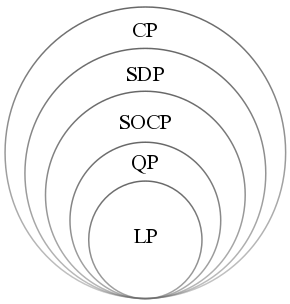
\includegraphics[width = 0.6\textwidth]{images/convex.png}
    \end{frame}

    \begin{frame}{Property}
      \begin{spacing}{1.5}
        \begin{itemize}
          \item Every local minimum is a global minimum.
          \item If the objective function is strictly convex, then the problem has at most one optimal point.
          \item Non-Convex $\to$ Convex
          \item Many methods can be used to solve and wide applications.
        \end{itemize}
      \end{spacing}
    \end{frame}

    \begin{frame}{Basic iterative approaches}
      \begin{itemize}
        \item \textcolor{yellow}{Line search}:
        \begin{enumerate}
          \item Compute a descent direction $p_k$
          \item Choose $ \displaystyle \alpha _{k} $ to 'loosely' minimize $ h(\alpha )=f(\mathbf {x} _{k}+\alpha \mathbf {p} _{k}) $ over $ \alpha \in \mathbb {R} _{+}$
          \item Update $ \mathbf {x} _{k+1}=\mathbf {x} _{k}+\alpha _{k}\mathbf {p} _{k} $, and $ {\textstyle k=k+1} $
          \item Until $ \|\nabla f(\mathbf {x} _{k+1})\| $ < tolerance.
        \end{enumerate}

        \item \textcolor{yellow}{Gradient descent}:
        \[x_{k+1}=x_k+\alpha_k d_k\]
        \[f(x_{k+1}) = f(x_k+\alpha_k d_k) < f(x_k)\]
        \item \textcolor{yellow}{Subgradient method}(for non-differentiable)
        \\
        Convergence conditions and Step size rules.
      \end{itemize}
    \end{frame}

    \begin{frame}{Gradient}
      Two essential elements: step size and descent direction. All kinds of methods are based on the fundamental.
      \begin{itemize}
        \item Random
        \item Batch
        \item Proximal gradient method
        \item Newton's Method
        \item Quasi-Newton method
      \end{itemize}
      convergence condition
    \end{frame}

    \begin{frame}{KKT}
      \[L(\mathbf {x} ,\mathbf {\mu } ,\mathbf {\lambda } )=f(\mathbf {x} )+\mathbf {\mu } ^{\top }\mathbf {g} (\mathbf {x} )+\mathbf {\lambda } ^{\top }\mathbf {h} (\mathbf {x} ) \]
      \quad where $ \mathbf {g} (\mathbf {x} )=\left(g_{1}(\mathbf {x} ),\ldots ,g_{m}(\mathbf {x} )\right)^{\top } $, $ \mathbf {h} (\mathbf {x} )=\left(h_{1}(\mathbf {x} ),\ldots ,h_{\ell }(\mathbf {x} )\right)^{\top }$.

      \begin{itemize}
        \item \textcolor{yellow}{Stationarity}

        $ f(x) $: $ \nabla f(x^{*})+\sum _{i=1}^{m}\mu _{i}\nabla g_{i}(x^{*})+\sum _{j=1}^{\ell }\lambda _{j}\nabla h_{j}(x^{*})=\mathbf {0}$
        \item \textcolor{yellow}{Primal feasibility}

        $ g_{i}(x^{*})\leq 0,{\text{ for }}i=1,\ldots ,m $
        $ h_{j}(x^{*})=0,{\text{ for }}j=1,\ldots ,\ell \,\! $
        \item \textcolor{yellow}{Dual feasibility}

        $\mu _{i}\geq 0,{\text{ for }}i=1,\ldots ,m $
        \item \textcolor{yellow}{Complementary slackness}

        $ \mu _{i}g_{i}(x^{*})=0,{\text{ for }}\;i=1,\ldots ,m. $

        When there are no inequality constraints, i.e.,$ m=0 $, the KKT conditions turn into the Lagrange conditions, and the KKT multipliers are called Lagrange multipliers.
      \end{itemize}
    \end{frame}

    \begin{frame}{Duality}
      \begin{equation*}
        \begin{align}
        f(x,\lambda)=& f_{0}(x)+\sum_{i=1}^{m}\lambda_{i}f_{i}(x) \\
        g(\lambda)=& \min_{x\in {\mathcal {D}}}  f(x,\lambda) \text{Concave}
      \end{align}
      \end{equation*}

      The dual function yields lower bounds on the optimal value $p^{*}$
      of the initial problem.

      \[ g(\lambda)\leq p^{*} .\]

      \[\max_\lambda \min_x f(x,\lambda) \leq \min_x \max_\lambda f(x,\lambda).\]

      Strong duality: $ d^{*}=\max _{\lambda \geq 0}g(\lambda)=\min f_{0}=p^{*}$.

      Constraint qualification such as Slater's condition holds.
    \end{frame}

    \begin{frame}{Other Methods}
      \Large
      \begin{spacing}{1.5}
        \begin{itemize}
          \item Interior-point method
          \item Penalty method
          \item Lagrange multiplier
          \item Augmented Lagrangian method
          \item Alternating Direction Method of Multipliers(ADMM)
        \end{itemize}
      \end{spacing}
    \end{frame}

    \begin{frame}{Non-Convex}
      \item convert to Convex
      \item heuristics
      The important thing is how to jump out of the local optimization.
      Change the parameter by experience.
    \end{frame}

    \begin{frame}{Random optimization}
      \item Methods
      \item Algorithmic idea
    \end{frame}
